\documentclass{beamer}

\usepackage[utf8]{inputenc}
\usecolortheme{beaver}
\usepackage{caption}
\usepackage{subcaption}
\usepackage{mathtools}
\usepackage{todonotes}
\usepackage{amsmath}
\usepackage{bm}
\usepackage{listings}
\usepackage{ragged2e}
\usepackage{titlecaps}
\usepackage{fancyvrb}

\def\ci{\perp\!\!\!\!\!\perp}

\newtheorem{proposition}{Proposition}
\Addlcwords{for a is but and with of in as the etc on to if}

\setbeamertemplate{section in toc}{\inserttocsectionnumber.~\inserttocsection}
\usetheme{Boadilla}
\makeatletter
\setbeamertemplate{footline}{%
    \leavevmode%
    \hbox{%
        \begin{beamercolorbox}[wd=.3\paperwidth,ht=2.25ex,dp=1ex,center]{author in head/foot}%
            \usebeamerfont{author in head/foot}\insertshortauthor\expandafter\beamer@ifempty\expandafter{\beamer@shortinstitute}{}{~~(\insertshortinstitute)}
        \end{beamercolorbox}%
        \begin{beamercolorbox}[wd=.55\paperwidth,ht=2.25ex,dp=1ex,center]{title in head/foot}%
            \usebeamerfont{title in head/foot}\insertshorttitle
        \end{beamercolorbox}%
        \begin{beamercolorbox}[wd=.15\paperwidth,ht=2.25ex,dp=1ex,right]{date in head/foot}%
            \usebeamerfont{date in head/foot}\insertshortdate{}\hspace*{2em}
            \insertframenumber{} / \inserttotalframenumber\hspace*{2ex} 
        \end{beamercolorbox}}%
        \vskip0pt%
    }
\makeatother

\begin{document}

\title[]{Expert-in-the-Loop Structure Learning}
\author{Ankur Ankan}
\date{}

\maketitle

\begin{frame}{Directed Acyclic Graphs (DAGs)}
	\todo[inline]{Add an example of a DAG here}
	
	\begin{itemize}
		\item Nodes represent random variables.
		\item Directed edges represent causal relationships.
		\item For eg., node1 has a direct effect on node2, node1 has an undirect effect on node3.
		\item Used for causal effect estimation.
	\end{itemize}
\end{frame}

\begin{frame}{Learning DAGs From Data}
	\begin{figure}
		\centering
		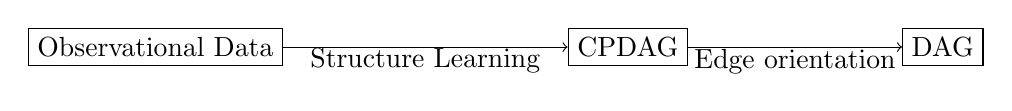
\begin{tikzpicture}
			\node[draw, rectangle] (x) at ( 0, 0 ) { Observational Data };
			\node[draw, rectangle] (y) at ( 6, 0 ) { CPDAG };
			\node[draw, rectangle] (z) at ( 10, 0) { DAG };
		
			\draw[->](x) -- (y) node[midway, below, yshift=0.1cm]{ Structure Learning };
			\draw[->](y) -- (z) node[midway, below, yshift=0.1cm]{ Edge orientation };
		\end{tikzpicture}
	\end{figure}
	\todo[inline]{Improve the figure. Show an example right below the steps }

	\begin{itemize}
		\item Causal Discovery/Structure Learning: Recover the true underlying DAG from observational data.
		\item Many class of algorithms such as constraint-based (PC, FCI), score based (Hill-Climb, GES), optimization-based (No Tears).
		\item However, algorithms can only recover the Markov Equivalence Class known as CPDAGs.
		\item To orient the edges of the CPDAG, we need to either use expert knowledge or make some assumptions.
	\end{itemize}
\end{frame}

\begin{frame}{Causal Discovery in Practice}
	\begin{itemize}
		\item Adaption of causal discovery is very limited.
		\item Researchers prefer to draw models by hand based on domain knowledge.
		\item Potential reasons could be:
			\begin{itemize}
				\item Algorithms can make obvious mistakes, making it harder to trust.
				\item Hard to choose an algorithm for a given dataset because of the different assumptions.
				\item No way to evaluate/compare algorithm performance on the given dataset.
			\end{itemize}
		\item However, some researchers do test their model after drawing.
	\end{itemize}
\end{frame}

\begin{frame}{Model Testing using Independence Tests}
	\todo[inline]{Add an example of model testing here}

	\begin{itemize}
		\item Test for missing edges in the model.
		\item If the test fails, it implies that the correlation between the variables is not explained by the model.
		\item The model is then modified to make it more agreeable with the data.
	\end{itemize}
\end{frame}

\begin{frame}{Human-in-the-loop Structure Learning}
	\begin{itemize}
		\item As most models are built by hand, a tool that can help with building these models with the help of testing.
	\end{itemize}
\end{frame}

\begin{frame}{Show an example of how this works}
\end{frame}

\begin{frame}{An effect size for mixed data}
\end{frame}


\begin{frame}{Empirical Analysis}
	\begin{itemize}
		\item Random DAGs on $ 10 $ nodes are generated.
		\item Data is simulated from these DAGs using linear models with random parameters.
		\item We use the simulated data to learn back the original model.
		\item We then compare the Structural Hamming Distance and Structural Intervention distance between the true and the learned graph.
		\item Because the structure learning algorithms can only learn the CPDAG, we show the best case and worst case DAGs.
	\end{itemize}
\end{frame}

\begin{frame}{Empirical Analysis}
	Need to simulate how an expert would use this to build DAGs.
	\begin{itemize}
		\item Take a greedy approach and choose the edge with the highest effect.
		\item After each edge addition the effects are updated.
		\item A pruning step is done to check if adding an edge removes some of the effects.
		\item An oracle is used to determine the direction of the edge. With some given confidence, the oracle either gives
			a correct answer or randomly.
	\end{itemize}
\end{frame}

\begin{frame}{Empirical Analysis: Structural Hamming Distance}
	\begin{figure}
		\centering
		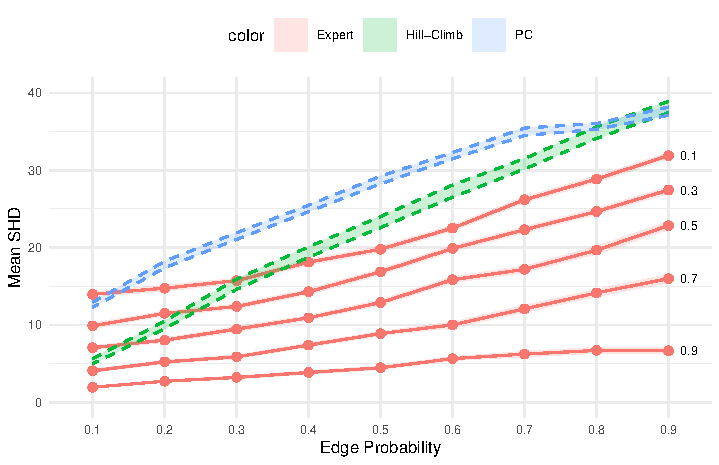
\includegraphics[scale=0.9]{../../2024-human-sl/code/plots/shd_ribbon.pdf}
		\caption{SHD vs edge probability}
	\end{figure}
\end{frame}

\begin{frame}{Empirical Analysis: Structural Hamming Distance}
	\begin{figure}
		\centering
		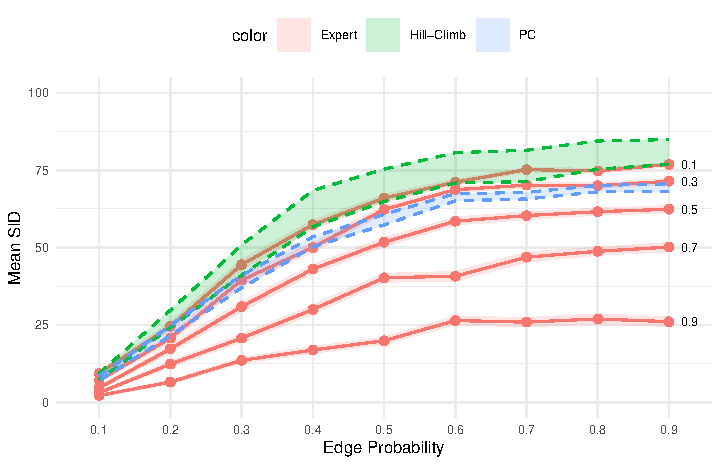
\includegraphics[scale=0.9]{../../2024-human-sl/code/plots/sid_ribbon.pdf}
		\caption{SID vs edge probability}
	\end{figure}
\end{frame}

\begin{frame}{Conclusion}
	\begin{itemize}
		\item We propose a tool to interactively draw DAGs combining it with testing.
		\item We propose an effect size measure for mixed data.
		\item For oracles with decent accuracy the method works well.
		\item Oracles can be replaced with LLMs.
	\end{itemize}
\end{frame}

\end{document}
